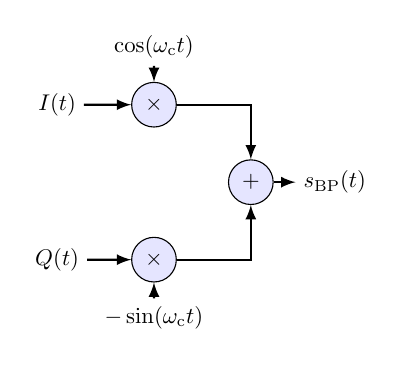
\begin{tikzpicture}[auto, >=latex, scale=0.82, every node/.style={scale=0.82}]
    \node (I) at (0,1.2) {$I(t)$};
    \node (Q) at (0,-1.2) {$Q(t)$};
    \node[draw,circle,fill=blue!10] (m1) at (1.5,1.2) {$\times$};
    \node[draw,circle,fill=blue!10] (m2) at (1.5,-1.2) {$\times$};
    \node (cos) at (1.5,2.1) {$\cos(\omega_\mathrm{c} t)$};
    \node (sin) at (1.5,-2.1) {$-\sin(\omega_\mathrm{c} t)$};
    \node[draw,circle,fill=blue!10] (sum) at (3.0,0) {$+$};
    \node (bp) at (4.3,0) {$s_\mathrm{BP}(t)$};
    \draw[->,thick] (I) -- (m1);
    \draw[->,thick] (Q) -- (m2);
    \draw[->,thick] (cos) -- (m1);
    \draw[->,thick] (sin) -- (m2);
    \draw[->,thick] (m1) -| (sum);
    \draw[->,thick] (m2) -| (sum);
    \draw[->,thick] (sum) -- (bp);
\end{tikzpicture}